\documentclass[a4paper,12pt,french]{article}

\usepackage[TD]{../../../Style}

% Début du document
%%%%%%%%%%%%%%%%%%%
\begin{document}

\titre{Exercices - Chapitres 1 à 3}

\begin{multicols*}{2}

\section*{Suites, généralités}

\begin{exercice} \
Soit $a$ la suite telle que $a_0=10$ et pour $n \in \N, a_{n+1}=a_n+10$.
\begin{enumerate}
\item Déterminer $a_1,a_2,a_3$.
\item Représenter les cinq premiers termes de cette suite sur un repère.
\item Emettre une conjecture concernant son sens de variations.
\end{enumerate}
\end{exercice}

\begin{exercice} \
Soit $g$ la suite telle que $g_0=1$ et pour $n \in \N, g_{n+1}=g_n \times 1.5$.
\begin{enumerate}
\item Déterminer $g_1,g_2,g_3$. On arrondira au dixième.
\item Représenter les cinq premiers termes de cette suite sur un repère.
\item Emettre une conjecture concernant son sens de variations.
\end{enumerate}
\end{exercice}

\begin{exercice}
On se donne la suite $u$ telle que $u_0=4$, et pour passer d'un terme au suivant, on multiplie par 2 et on retire 3.
\begin{enumerate}
\item Recopier et compléter le schéma suivant:
\begin{centrer}
\resizebox{\linewidth}{!}{
\hspace{-10mm}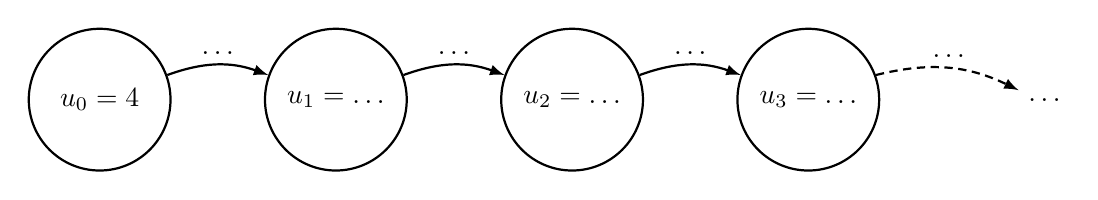
\begin{tikzpicture}[scale=1]
\node[draw,circle,thick, minimum size=18mm] (W0) at (-3,0) {$u_0=4$};
\node[draw,circle,thick, minimum size=18mm] (W1) at (0,0) {$u_1=\ldots$};
\node[draw,circle,thick, minimum size=18mm] (W2) at (3,0) {$u_2=\ldots$};
\node[draw,circle,thick, minimum size=18mm] (W3) at (6,0) {$u_3=\ldots$};
\node (W4) at (9,0) {$\ldots$};
\draw[->,>=latex,thick] (W0) to[bend left=20] node[midway,above]{$\ldots$} (W1);
\draw[->,>=latex,thick] (W1) to[bend left=20] node[midway,above]{$\ldots$} (W2);
\draw[->,>=latex,thick] (W2) to[bend left=20] node[midway,above]{$\ldots$} (W3);
\draw[->,>=latex,thick,densely dashed] (W3) to[bend left=20] node[midway,above]{$\ldots$} (W4);
\end{tikzpicture}}
\end{centrer}
\item Recopier et compléter: $u_{n+1}=\ldots u_n - \ldots$
\item En utilisant la calculatrice, déterminer $u_{20}$.
\end{enumerate}
\end{exercice}

\section*{Fonctions affines}

\begin{exercice}
Sur un repère, construire les droites $d_1$ et $d_2$ d'équations respectives $y=3x-2$ et $y=-\frac 3 5 x+4$.
\end{exercice}

\begin{exercice}
Lecture
\end{exercice}

\begin{exercice}
tableau signes
\end{exercice}

\begin{exercice}
Détermination algébrique
\end{exercice}

\section*{Fonctions de degré 2}

\begin{exercice}
Donner une fonction, dire a,b,c puis identifier a laquelle elle correspond parmi 2 paraboles et pourquoi. Tracer l'axe de symétrie, placer le sommet.
\end{exercice}

\begin{exercice}
Relier 3 équations à 3 paraboles du type $y=ax^2+c$.
\end{exercice}

\begin{exercice}
Déterminer l'équation d'une parabole du type $y=ax^2+c$
\end{exercice}

\begin{exercice}
Une parabole, déterminer les racines graphiquement puis dresser le tableau de variations. Donner le signe de a. Calculer les coordonnées du sommet et vérifier en le plaçant.
\end{exercice}


\end{multicols*}
\end{document}
